
\begin{savequote}
Verbal and nonverbal activity is a unified whole, and theory and methodology should be organized or created to treat it as such.
\qauthor{Kenneth L. Pike}
\end{savequote}

\chapter[The LILiR TwoTalk Corpus and Annotation Data]{The LILiR TwoTalk Corpus and Annotation Data}
\label{ChapterCorpus}

\thesiscomment{MAIN POINT: Because NVC is dependent on social situation and no appropriate database is available, we record and annotate a new NVC database that has minimum experimental constraints and annotated using high dimensional labels.}

\thesiscomment{WHAT we do}

\thesiscomment{HOW we do it}

\thesiscomment{RESULTS, IMPACT and NOVELTY}

\ac{NVC} occurs as a component of almost all forms of human communication. In order to study it, it is usually convenient to record a representative sample of human communication for later analysis. This set of data is called a ``corpus''. The observations in the corpus are usually labelled by a group of observers or annotators. 
%Annotations are used to systematise the content in the corpus to facilitate further analysis. 
The manner of recording and the type of annotation is dependent on the behaviour under investigation. This chapter describes the collection of a new corpus that occurs during informal conversations. Minimal experimental constraints are used in order to retain the natural and spontaneous characteristics of informal conversation. %However, the recorded sessions were conducted in a studio environment between pairs of selected participants, which may differ from informal conversations in the field.

The corpus described in this chapter has been named the LILiR TwoTalk corpus\footnote{The name derives from this work being associated with the EPSRC LILiR project.}. 
%At the time of recording, there were no similar publicly available \ac{NVC} data sets that were naturalistic (non-role play or otherwise contrived by the experimenter), suitable for tracking and spontaneous\footnote{This is discussed further in Section \ref{SectionExistingDataSets}}. 
At the time this work was conducted, there were limited appropriate data sets that were publicly available. Corpuses have been recorded in various situations with a range of spontaneity and naturalness. The most viable candidate was the AMI meeting corpus \cite{Carletta2007}. However, only a portion of this corpus is naturalistic and it was not suitable for the feature tracking method employed in Chapter \ref{ChapterClassification} and subsequent chapters. This chapter describes a new corpus that was designed specifically to fit the requirements of this study.

Posed data differs from spontaneous data in many ways because \ac{NVC} signals are dependent on social context\footnote{Even if posed data is considered as having no social context, the absence of a social context is a factor in \ac{NVC} expression.}. Informal conversations can be recognised in other cultures because they have some characteristics that are cross-cultural. The choice of a common, reproducible social situation is attractive for cross cultural study. The social situation of informal conversation is easy to organise and reproduce experimentally. However, spontaneous data is challenging to annotate because of the \ac{NVC} signals being sparsely distributed throughout lengthy videos. Also, there is no clear application for informal conversation behaviour recognition at this time apart from further improving our understanding of human behaviour.
%This corpus is used in later chapters of this thesis for training an automatic system. 
Previous annotation approaches have focused on encoding a subject's internal state, emotions, gestures, dialogue acts, social relationships, topic, attention or expressions. The LILiR TwoTalk corpus uses annotation labels that encode the communicative non-verbal behaviour \cite{Ekman1969}, including both the verbal and \ac{NVC} aspects. 
%The labels of overall meaning provide a basis for an investigation into the association between \ac{NVC} gestures and communication meaning.

The main contributions of this chapter are:

\begin{itemize}
 \item a new corpus of informal conversations between pairs of people which is suitable for the study of \ac{NVC} signals,
 \item an annotation set of communicative non-verbal behaviours. The annotation was performed using a new set of \ac{NVC} quantised, dimensional labels,
 \item inter-annotator agreement of the collected data was analysed and 
 \item co-occurrence of \ac{NVC} signals was found and
 \item the recordings and annotation data are publicly
 available\footnote{\scriptsize{http://www.ee.surrey.ac.uk/Projects/LILiR/twotalk\_corpus/}}.
\end{itemize}

The next section provides an overview of recording conditions, annotation systems and related work. The recording of the new corpus is described in Section \ref{SectionDataCapture}. Section \ref{SectionDescribeQuestions} describes the questionnaire used by the annotators. Section \ref{SectionMultiCultitureAnnotation} describes how multiple annotators rated the corpus video samples. Demographics of the annotators are described in Section \ref{SectionAnalysisOfHumanAnnotation} and Section \ref{SectionAnalysisOfMeanRatings} investigates patterns occurring in the annotation data.

\section{Related Research}
\label{BackgroundCorpus}

This section describes the creation and use of corpuses that can be used as the basis for computer based analysis. The most significant social situations and annotation systems are discussed, as well as the existing data sets. %The situation in which a corpus is recorded, if used to train an automatic recognition system, determines in which situations the system may be deployed effectively.

%An early use of video recording to study \ac{NVC} was performed by Condon and Ogston \cite{Condon1971} in which the material was replayed slowly to allow better manual observation. More recently, the use of computers enables some types of human behaviour to be analysed automatically, and patterns can be found that are difficult for humans to manually identify.

%Practical guidance on recording \cite{Frank2005}
%High level look at factors in designing human databases \cite{Cowie2008}
%Emotaboo design considerations \cite{Zara2007}, also EmoTV \cite{Devillers2008}, \cite{Afzal2009}, FreeTalk \cite{Campbell2010}, B3D(AC)\^2 \cite{Fanelli2010b}, D64 \cite{Oertel2010}

\subsection{Social Context}
\label{BackgroundSocialContextUsedInTwoTalk}

%Context is important for literal meaning too \cite{McHoul08}
% Review of data sets, etc \cite{Cowie2005}
%Other acted data set use \cite{Smith2005}, \cite{SobolShikler2010}, FERA \cite{Tariq2011}, movie extracts \cite{Kipp2009}
%Meeting, AMI corpus , \cite{Hillard03}, \cite{Petridis2010}, \cite{Truong2009}
%Interview \cite{Grimm2007}, \cite{Kanluan2008}, \cite{Devillers2008}

Acted corpuses are convenient to use because the samples have a predetermined ground truth and little recording time is wasted on uninteresting behaviour. It is impossible to predict or control the specific behaviours that will occur in naturalistic behaviour, and therefore videos require annotation to determine the labels. The sections of the video that are of interest to researchers may be unevenly distributed. Contrived situations, such as role play, tasks and games are an intermediate approach, in which participants are guided by the experimenter to maximise the useful content and allow for natural reactions to unnatural stimuli. As discussed in Section \ref{BackgroundWhatFactorsInfluenceNvc}, the situation in which a corpus is recorded affects the behaviours that occur. 
%The type of situation in which a corpus is recorded should be driven by the intended application of the final system. 
%This section will review some of the common contexts used for recording corpus data, and some background on the informal conversational context.

Historically, a large amount of emotion recognition research has been conducted on acted data sets, in which participants are told to express or pose particular behaviours, or the behaviour is expressed in a contrived or rare social situation. Often, a sequence starts and ends with a neutral expression. However, spontaneous emotion can change without transitioning through a neutral expression. Novel methods continue to be proposed for acted data sets \cite{Chew2012b}, including: {BU-3DFE} \cite{Moore2009}, {JAFFE} \cite{He2005}, Mind Reading {DVD} \cite{Kaliouby2005} \cite{SobolShikler2010} and {GEMEP}-{FERA} \cite{Valstar2011}. Emotion recognition based on basic emotions is generally considered a solved problem \cite{Valstar2012}. Many studies are based on elicited emotional responses from subjects that are interacting with a device being controlled by the experimenter \cite{Afzal2009}, e.g. viewing videos \cite{Sun2004, Pfister2011}, interacting with computer characters (e.g. SAL) \cite{Wollmer2009} or a robot \cite{Seppi2008}. This method is also referred to as a ``Wizard of Oz'' situation. Further naturalism is added by having a social situation with two or more humans participating in a task. Data can be recorded in a game environment, such as EmoTaboo \cite{Zara2007}, interviews \cite{Cowie2009} or in a niche social situation, such as speed dating \cite{Madan2005}. Contrived social situations, in which participants spontaneously react to an experimenter designed social situation, include staged interviews \cite{Zeng2006} or meetings, such as in the majority of the AMI meeting corpus \cite{Carletta2007} for which approximately ''two-thirds of the data has been elicited using a [role-play] scenario'' \cite{amiproject}. Few studies consider social situations that are not contrived or goal based activities. Almost all studies occur in the laboratory, due to the practical difficulty of recording natural social situations. Controlled situations can be useful for data collection if the automatic system is intended to be deployed in such an environment. %Given the need for naturalistic data, it might be advantageous to select a common social situation, such as informal conversation, that contains rich and diverse \ac{NVC}.

Informal conversations are used throughout this thesis. An informal conversation is a common social situation and one which almost everyone experiences on a daily basis. This context is also referred to as ``casual conversation'' or as ``chatting''. These conversations are usually relaxed, unfocused discussions about trivial matters. Eggins and Slade \cite{Eggins1997} defines casual conversation as ``talk which is NOT motivated by any clear pragmatic purpose''. This social context has not received much attention from linguists or from the human behaviour recognition community. Humphrey claimed that casual chatting can be recognised across cultures because of the activity's characteristics \cite{Humphrey1993} which are:

\begin{itemize}
 \item being informal,
 \item lacking focus,
 \item containing haphazard reiteration and
 \item having ``topics of conversation crumble away in the compulsion of people saying what they can't help saying''.
\end{itemize}

Automatic recognition of \ac{NVC} in informal conversations is attractive for a number of reasons. Informal conversation is a specific social situation that is relatively easy to replicate (specifically, the social context can be staged relatively easily). It is also commonly occurring, cross cultural and occurs in almost all social groups.

However, there are potential drawbacks compared to other approaches:

\begin{itemize}
 \item the frequency of strong emotion and intense \ac{NVC} is relatively low,
 \item there are times in which the participants are passive, which contains little information of interest and
 \item labelling must be performed by annotators.
\end{itemize}

The annotation of the data is discussed in the next section.

\subsection{NVC Annotation, Questionnaire Design and Labels}
\label{BackgroundWhyNvcAnnotationIsBoring}
\label{BackgroundMultipleAnnotation}
\label{BackgroundQuestionaireDesign}

Annotation uses human observers to review and provide judgements regarding the content of the corpus. Video clips are viewed by each annotator and rated based on questions set by the experimenter. The purpose of annotation is to record the way the corpus is perceived by the annotators and thereby provide a basis to study the content of the corpus.

%NVC annotation difficult 

Many factors influence the perception of \ac{NVC} signals (see Section \ref{BackgroundWhatFactorsInfluenceNvcPerception}). For annotation of a corpus, these factors are still present but can be somewhat controlled. Studies have focused on the annotation perception issue, in an attempt to reduce inter-annotator disagreement and to improve the quality of the data. Reidsma claimed that inter-annotator agreement is caused by poorly chosen annotation concepts and annotation schema, clerical errors, lack of annotator training, as well as context \cite{Reidsma2008}. His thesis is currently the broadest review of the annotator agreement issue. Experts can be more consistent than untrained observers for some annotation tasks, e.g. high quality \ac{FACS} \cite{Donato1999}. Annotation can be improved by showing the video leading up to an emotion \cite{ElKaliouby03}, as well as showing them the entire corpus before starting to annotate \cite{Hoque2009}. Studies have noted that inter-annotator agreement was lower for stylised emotion than for spontaneous emotion \cite{Bernhardt07, Afzal2009b}. Annotation labels that require less interpretation might be thought of as advantageous because they have higher inter-annotator agreement \cite{Fasel2003}, but this avoids the problem of perceptual differences which needs to be addressed for effective \ac{NVC} recognition.

Annotation of emotion data sets have often been performed by multiple observers. The annotators use a task specific encoding system that is selected or designed by the experimenter. These annotations are usually combined to form a consensus score, either by taking the majority vote in the case of discrete classes \cite{Seppi2008, Escalera2009}, or taking the mean in the case of dimensional variables \cite{Wollmer2008, Mower2009}. In this case dimensional is defined as ``the range over which or the degree to which something extends'' \cite{merriamwebster}. This is done to reduce the effect of different interpretation among the annotators and emphasise the generally agreed content of the corpus. However, this attempt to minimise the role of interpretation differences makes the ground truth differ from the individual human observations. A less common approach is to consider subsets of annotators and model them individually. A subset of annotators that had inter-agreement was modelled by Reidsma and op den Akker \cite{Reidsma2008b}. Groups of annotators can be collected and handled separately, as in the case of naive and expert annotators \cite{Donato1999}. Although judgement based annotation is almost universally used, a few studies have used self assessment \cite{Madan2005} or a combination of self-assessment and annotator judgements \cite{Hoque2009}. 
%We have discussed how selection of corpus data and annotators is important for useful annotation data. 
%The choice of encoding schemes, including labels and discrete/continuous scales selection, will now be reviewed.

%The choice of annotation label used is important in determining the possible applications for the data. 
There are many pre-existing annotation systems that encode facial expression, emotion, mental states, affective state, gesture, dialogue acts, social relationships, attention and communication. These systems can be broadly grouped into four classes: those that assess the internal state of a person, a person's physical behaviour, social dynamics between people and those that describe the meaning of specific actions. Emotion labelling is one of the most popular facial or mental state labelling systems. The most common emotion labelling system is based on discrete classes, occasionally using the original Ekman 6 basic emotions \cite{Cohen2000}. There are no commonly agreed set of emotions and the choice of appropriate labels would depend on the intended application. Discrete emotional classes cannot comprehensively cover all emotional states and instead focus on episodic occurrences \cite{Cowie2005} while ignoring pervasive emotion. Pervasive emotions are emotional states that are routinely experienced in life but not present in an emotionless state. 

Emotion labelling has often been expressed in a dimensional, abstract 2{D} space such as activation and evaluation \cite{Cowie2000} or valence and activation \cite{Cowie1999, Liscombe2003, McRorie2007}. In this case, abstract means ``non-prototypical'' and ``defined in terms of natural language'' \cite{Kazemzadeh2013}. It is unclear how many dimensions are necessary to faithfully encode human perception of \ac{NVC} or emotion. A 2{D} space may not be enough to encode all emotions unambiguously \cite{Fontaine2007}. Schr\"{o}der \etal claimed that emotion could be effectively encoded using only 2 dimensions \cite{Cowie2000} in a system such as ``FeelTrace'', but they admit there was ambiguity in distinguishing between anger and fear. However, dimensional encoding is not limited to these labels: Ashraf \etal \cite{Ashraf2007} used a dimensional scale for rating pain, Mikels \etal \cite{Mikels2005} collected emotional annotation data for images using \textit{fear}, \textit{sadness}, \textit{disgust}, and \textit{anger}, each measured on independent, 7 point Likert scales and Ball and Breeze \cite{Ball2000} using dominance and friendliness dimensions to encode personality. Dimensional scales have also been used to rate toddler behaviour \cite{Lorber2003}, facial action intensities \cite{Fasel2000}, happiness and sadness \cite{Hsee1992}, classroom interactions\footnote{http://www.teachstone.org/about-the-class/} and non-verbal behaviour \cite{Feldman1991}. The diversity of labels used in dimensional systems is broad to cover the variety of scientific problems to be addressed.

The AMI corpus includes many types of annotation labels including dialogue acts, attention and specific gestures \cite{Carletta2007}. The annotation was later expanded with dominance \cite{Aran2010} and emotion. Devillers \cite{Devillers2008} used a different labelling system based on appraisal theory \cite{Scherer1999}, in which the emotion stimuli are rated rather than the mental state.

%Other emotion labelling examples  \cite{Dornaika2005} \cite{Abrilian2006} \cite{Hong2006} \cite{Wang2006} \cite{Zeng2006} \cite{Lee07} \cite{Datcu2007} \cite{Grimm2007} \cite{Moore07} \cite{Zara2007} \cite{Kanluan2008} \cite{Seppi2008} \cite{Moore2009} \cite{Mower2009} \cite{Fanelli2010b} \cite{SobolShikler2010} \cite{Tariq2011} \cite{Nicolaou2011}
%other Ekman based \cite{Feng2005}
%other abstract \cite{Cowie2000}, 

Various encoding systems have been discussed but the choice of the most appropriate system is dependent on the type of behaviour of interest to the experimenter. Annotation labels can focus on either the internal mental state or the intentional communication but not usually both. An example of labels that focus on internal states is the Mind Reading corpus, originally created to assist autistic observers to recognise a mental state in others. This was applied to automatic recognition by el Kaliouby and Robinson \cite{ElKaliouby2004} for a subset of labels: agreeing, concentrating, disagreeing, interested, thinking and unsure, with the emphasis on mental state. Afzal \etal used similar affect labels for recognition \cite{Afzal2009b}. Pain has also been used for annotated and automatic recognition \cite{Ashraf2007, Lucey2009}. 

Annotation labels which focus on verbal communication meaning can also be applied to \ac{NVC}. Hillard and Ostendorf \cite{Hillard03} performed classification using agreement and disagreement labels on intentional verbal utterances. Zara \etal \cite{Zara2007} used high level groupings of verbal communication acts in EmoTaboo, some of which correspond to a meaningful communication. Bavelas and Chovil \cite{Bavelas97} counted the frequency of meaningful facial gestures. 
%The other labelling systems that have been used for automatic system training have focused on mental states, expression or gesture.

Another group of human behaviours that are of interest to researchers is facial expression. Facial expressions are an externally observable movement of the body which require less interpretation than emotion to annotate. This is in contrast to emotions which largely occur in the mind and only sometimes manifest themselves in behaviour or expression. 
%A facial expression can be associated to an \ac{NVC} meaning or emotion but this association is dependent on context. 
The most popular method for encoding facial expression is the \acf{FACS} \cite{Ekman1978}, in which facial \acf{AU}s correspond to sets of muscles. \ac{FACS} is widely used for labelling expressions and has been used as the basis for regression systems (\cite{Savran2012}), although most papers only use a subset of \ac{FACS}. However, \ac{FACS} annotation exhaustively encodes expressions, requires trained observers and is very time consuming to perform. The encoding is typically based on binary classes and does not consider the intensity of expression. 
%This loss of information may be significant for some applications, such as lip reading. 
Others have used expression labels that did not use the \ac{FACS} system, for example Kanaujia \etal \cite{Kanaujia2006} labelled nodding and blinking.

%other FACS based labelling \cite{Bartlett2006} \cite{Tang2007} \cite{Zhu2009} \cite{Tax2011} \cite{Taheri2011} \cite{Girard2011} \cite{Jeni2011} \cite{Valstar2012}

There are other facial analysis labelling approaches that do not fit with the previously discussed groups but have some relation to \ac{NVC}. Deception and truthfulness modifies the perception of communication and have been used as labels and in recognition \cite{Tsiamyrtzis07, Pfister2011}. 
%Naturalistic deception is not an intentional action and is therefore not a communication act. 
The outcomes of speed dating was labelled and recognised \cite{Madan2003} and this again is largely based on perception of \ac{NVC}, but the labels themselves do not correspond to meaningful communication. 
%Labels-laughter \cite{Petridis2008} \cite{Petridis2009} \cite{Truong2009} \cite{Petridis2010}
%Labels-identity \cite{Mok2004} \cite{Fang2009}
%Labels-social-dynamic \cite{Escalera2009}
Given that the situation in which data is recorded is significant, the next section discusses why a new naturalistic data set is needed for studying occurrences of meaningful \ac{NVC} signals.

\subsection{The Need for a Naturalistic Corpus}
\label{BackgroundNeedNaturalistic}

\thesisstatement{Recording social situation while seated in the lab and with no constraints on conversation topic provides data useful for studying social interactions (compromise between spontaneous conversations and getting useful data).}

\thesisstatement{Literature suggests significant differences in posed vs. natural human interaction}

\thesisstatement{Classifying naturalistic data is harder than posed data \cite{Akakin2011}}

There has long been criticism of the study of social phenomena in a laboratory environment. Although a laboratory is intended to assist the control of experimental variables, Argyle \cite{Argyle1975} claimed that too often study subjects ``sit in cubicles by themselves, watch flashing lights and press buttons; often there is no verbal communication, no NVC, no real motivation, and there are no situational rules''. Moving a social situation from its normal location to the laboratory can have significant effects, due to the subject's knowledge that they are being recorded \cite{Beattie1982b} but ethical and practical considerations make this fact hard to conceal \cite{Frank2005}. Posed and spontaneous data also have significant differences. If meaning in communication is the subject of study, context is significant which makes posed or over simplified data unsuitable \cite{Bavelas97}. However, not all human related research needs to be naturalistic and researchers need to assess the suitability of any database \cite{DouglasCowie2003}. Many emotion recognition systems have used posed data and this seems unlikely to change. However, different recording conditions have been shown to result in different behaviours. If an automatic system is trained based on a corpus and deployed in a different environment, it is quite possible that human behaviours will be significantly different and the automatic system will have poor performance. For example, the timings of natural and posed emotions are different \cite{Cohn2004}. This difference is so significant that posed and spontaneous examples of emotions can be manually and automatically distinguished \cite{Valstar2006, Pfister2011b}. Strong emotion is rarely expressed or is expressed in unusual circumstances, making recording of naturalistic examples difficult \cite{Cowie2008}. For natural data, the information content is unevenly distributed in time \cite{Cowie2009}. Rapid emotional transitions are more common in natural data than in posed data \cite{McRorie2007, Bavelas97}. Rapidly changing emotion has higher annotation demands and less predictability in recognition. Cowie \cite{Cowie2008} reviewed these issues in the context of creating databases suitable for human behaviour and concluded the challenges for recording and annotating such a database are significant, but stressed that these issues must be addressed to make progress. An alternative to using naturalistic data as the basis for automatic systems is to use data ``of a kind that might have to be dealt with in an application'' \cite{Cowie2009b}. In recent research, these types of datasets are becoming more popular. It is likely that some applications of \ac{NVC} recognition require the use of naturalistic data and this remains the focus of this thesis. 
%Given the need for naturalistic data, the next section reviews the existing data sets, focusing on naturalistic corpuses.

\subsection{Existing Data Sets}
\label{SectionExistingDataSets}

The majority of facial analysis and human behaviour data sets have focused on emotion or expression recognition. As discussed in the previous section, there is a need to use natural data, therefore many of the existing data sets are not appropriate for \ac{NVC} recognition. The existing naturalistic, public databases will be reviewed and the reasons for recording a new data set will be discussed in this section.

\begin{itemize}
\item \textit{Belfast Naturalistic Emotional Database} is a corpus using both television programmes and interviews \cite{Cowie2005}. The clips are between 10 and 60 seconds in duration. The variability of social context would make expression of \ac{NVC} rather diverse. Also, some of the social situations are rare, such as being an interviewee on a television programme.
\item \textit{EmoTV} comprises of 89 television interview monologues. The duration of video clips varies between 4 and 43 seconds. Again, the variability of social context is an issue, as well as the low quality of analogue broadcast TV. \cite{Devillers2008}
\item \textit{FreeTalk} is a four person conversation which was not limited in topic. Participants remained seated throughout. The conversation was conducted in a laboratory. This corpus is similar to the one presented in this chapter but FreeTalk was publicised after the TwoTalk corpus was recorded and used \cite{Campbell2010}.
\item \textit{D64 Multimodal Conversational Corpus} used unrestricted, multi-person conversation in a domestic environment \cite{Oertel2010}. This corpus is a significant improvement on previous data sets in that it recorded casual conversation outside of the laboratory environment. The subjects could move around or leave as desired. This data set was also publicised after the corpus in this chapter was recorded and used.
\end{itemize}

Although not the primary focus of this thesis, existing non-naturalistic datasets include:

\begin{itemize}
\item \textit{Canal9} is a series of broadcast television political debates between 2 or more participants and a moderator. This corpus is discussed in more detail in Section \ref{SectionCanal9}.
\item The majority of the \textit{AMI Meeting corpus} is a series of recordings of role play meetings in a group of 4 people. Approximately two thirds of the meetings are role play scenarios, and the remainder are naturalistic. People occasionally moving from seated to standing (Figure \ref{FigureAmiMeetingStanding}).
\item \textit{EmoTaboo} is a set of recordings of role play games between two participants.
\item \textit{MMI} is a searchable database of posed and elicited emotions.
\item \textit{Mind Reading} corpus is a library of short, silent videos of mental states performed by actors. This was originally produced as training material management of autism spectrum disorders. This corpus is described in more detail in Section \ref{SectionMindReading}.
\item \textit{Sensitive Artificial Listener (SAL)} is a corpus of elicited emotion based on a human interacting with a computer character that exhibits one of a set of personality types.
\item \textit{Green Persuasive Dataset} is a series of recordings of a role play situation between an experimenter and a volunteer with the discussion topic focused on environmental issues. The experimenter attempts to persuade the volunteer to adopt a more environmentally sustainable lifestyle.
\item \textit{MHi-Mimicry-db\cite{Sun2011}} is a 15 camera, 3 microphone recording of dyadic conversations. The participants were either in a political debate (34 recordings) or in a role-playing game (20 recordings).
\end{itemize}

\begin{table}
\centering
\caption{Summary of data sets used for emotion and conversation oriented research.}
\tiny
\begin{minipage}{0.99 \columnwidth}
\begin{tabular}{ | c | c | c | c | c |}
\hline
Corpus & Duration & Context & Participants & Labels \\% & Availability \\
\hline
Belfast Naturalistic \cite{Cowie2005} & 86 min labelled & emotional & Dyadic & Emotion  \\%& Subset is public \\ %(Feeltrace)
& 12 min available & interview & & \\
\hline
EmoTV \cite{Devillers2008} & 89 clips, 12 minutes & interview monologues & Monologue & Various \\% & Proprietary \\
\hline
FreeTalk \cite{Campbell2010} & 270 minutes & lab, conversation & 4 person & Various \\% & Public \\
\hline
D64 Multimodal \cite{Oertel2010} & 8 hours & domestic, conversation & 4-5 people & Unknown \\% & ? \\
\hline
Canal9 \cite{Vinciarelli2009}& 42 hours & debate & 2 to 4 person & Shots, ID \\% & Public\\
& & & \& moderator & \\
\hline
AMI Meeting \cite{Carletta2007}& 100 hours & Role play meeting& 4 people & Various \\% & Public, hi quality video on DVD\\
\hline
EmoTaboo \cite{Zara2007}& 8 hours & Mime game & Dyadic & Emotional Events\cite{Devillers2008} \\%& By arrangement\\
\hline
MMI \cite{Valstar2010}& Increasing with time & Various induced & Single participant & Various \\% & Public\\
\hline
Mind Reading\footnote{http://www.jkp.com/mindreading/} & \textasciitilde19 minutes & Posed & 1 Actor & Mental state \\% & Commercial\\
\hline
SAL \cite{Schroder2011}\footnote{http://semaine-db.eu/}& \textasciitilde10 hours & Wizard-of-OZ & 1 person & Emotion \\% & Available on CD\\ %(Feeltrace)
& & & with computer & \\
\hline
Green Persuasive& videos 25-48 minutes & role-play & dyadic & persuasiveness \\% & Public\\
Dataset\footnote{http://green-persuasive-db.sspnet.eu/} & 8 dyads & & & \\
\hline
MHi-Mimicry-db\cite{Sun2011} & \textasciitilde12 hours & discussion/role play & 40 people, dyadic & various \\
\hline
\end{tabular}
\end{minipage}
\normalsize
\label{TableAvailableDatasets}
\end{table}

\begin{table}
\centering
\caption{Summary of adverse factors for the suitability of existing datasets.}
\tiny
\begin{minipage}{0.99 \columnwidth}
\begin{tabular}{ | c | l |}
\hline
Corpus & Suitability \\
\hline
Belfast Naturalistic \cite{Cowie2005} & Staged interview, only a \textasciitilde12 min subset is available \\
& not labelled for \ac{NVC}, face size is small (approximately 150 by 200 pixels) \\
\hline
EmoTV \cite{Devillers2008} & Not publicly available \\
\hline
FreeTalk \cite{Campbell2010} & Video is small and faces are approximately 18 by 18 pixels \\
& unsuitable for tracking, only publicly available recently (since 2010) \\
\hline
D64 Multimodal \cite{Oertel2010} & not publicly available at time of writing \\
\hline
Canal9 \cite{Vinciarelli2009}& Unusual social situation, only a subset is annotated \textasciitilde10 min \\
 & not continuous view of subject, low quality interlaced broadcast video,\\
 & standing multiple participants may result in larger head pose changes \\
\hline
AMI Meeting \cite{Carletta2007}& Mostly contrived role play scenario \\
& although some meetings are naturalistic, \\
& not \ac{NVC} annotated, emotion annotations are not publicly available \\
& multiple participants may result in larger head pose changes \\
& and more complex interactions, video is highly compressed, \\
& face size is small (typically 110 by 70 pixels), \\
& contains a mixture of standing and seated behaviour \\
\hline
EmoTaboo \cite{Zara2007}& Not publicly available \\
\hline
MMI \cite{Valstar2010}& Focused on posed and induced expression not \ac{NVC} \\
& Only uses a single participant and not dyadic\\
\hline
Mind Reading& Acted, low quality video, face only 100 by 150 pixels, focuses on mental states not \ac{NVC} \\
\hline
SAL \cite{Schroder2011}& Human to computer character conversation rather than human to human conversation \\
& Available since Mar 2009 \\
% \hline
\hline
Green Persuasive& Contrived social situation, available since 2009, \\
Dataset & Small videos with face approximately 104 by 145 pixels\\
\hline
MHi-Mimicry-db\cite{Sun2011} & staged discussions or role-playing games, \\
& labelled for facial expression not \ac{NVC}, only recently available (since 2011)\\
\hline
\end{tabular}
\end{minipage}
\normalsize
\label{TableDatasetSuitability}
\end{table}

\begin{figure}
\centering
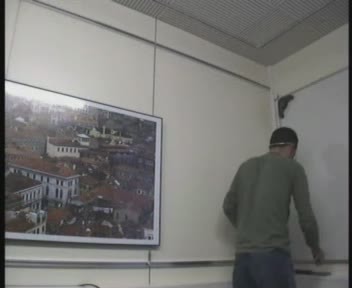
\includegraphics[width = 0.50 \columnwidth]{corpus/amimeeting-standing.jpg}

\caption[A participant getting up from a seated position in the AMI Meeting corpus]{An instance in the AMI Meeting corpus of a participant getting up from a seated position and standing near a white board with their back facing the camera (in video IN1014.Closeup2.avi frame 5200). This behaviour makes facial tracking problematic.}
\label{FigureAmiMeetingStanding}
\end{figure}

There are many other task based or induced emotion corpuses (see Table \ref{TableAvailableDatasets}), but they exhibit greater variability in social context, low video quality or the task being too specific make these data sets unsuitable. See Table \ref{TableDatasetSuitability} for the suitability of each data set. Also, many corpuses use more than two participants but limiting conversations to two persons is likely to be simpler to understand and analyse. Corpus videos in which the face has a small size can be difficult to accurately track. Corpus videos that feature more than two participants may have a larger head pose variation due to people turning to face different people during the conversation. These factors can make tracking less effective. Later chapters use Canal9 and Mind Reading for regression (see Sections \ref{SectionCanal9} and \ref{SectionMindReading}), but this thesis is primarily focused on a new \ac{NVC} corpus TwoTalk.
%No naturalistic corpus has \ac{NVC} annotation, which is at least as challenging as recording a suitable data set. 
The next section describes how the TwoTalk corpus was recorded.

%Naturalistic corpus from TV \cite{Devillers2008} 
%Survey paper \cite{Vinciarelli2008} 
%Good list of naturalistic databases \cite{Afzal2009} 

\section{Description of LILiR TwoTalk Corpus}
\label{SectionDataCapture}
\label{SectionDescriptionOfTwoTalkCorpus}

%This section describes how the ``LILiR TwoTalk Corpus'' was recorded and how the selection of video samples was performed. 
%As described in Section \ref{BackgroundNeedNaturalistic}, naturalistic data should have minimal experimenter constraints. 
Two participants were selected from the department and invited to a data capture session in a visual media lab. The only criteria used to select participants was the requirement to have people of roughly equal social seniority. Culture, familiarity and gender were not controlled in participant selection. However, these differences may affect the type and frequency of \ac{NVC} signals.

\begin{figure}
\centering
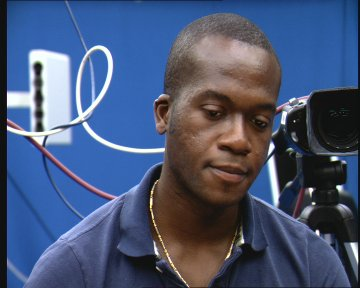
\includegraphics[width = 0.24 \columnwidth]{corpus/1008.jpg}
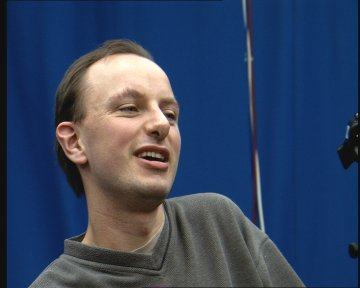
\includegraphics[width = 0.24 \columnwidth]{corpus/1011.jpg}
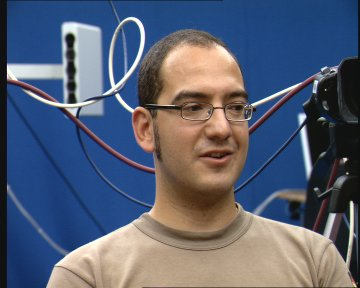
\includegraphics[width = 0.24 \columnwidth]{corpus/2008.jpg}
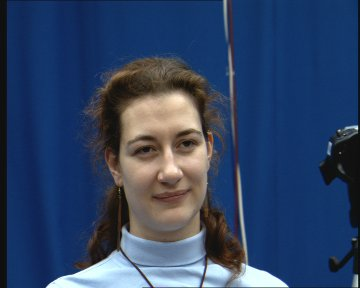
\includegraphics[width = 0.24 \columnwidth]{corpus/2011.jpg}

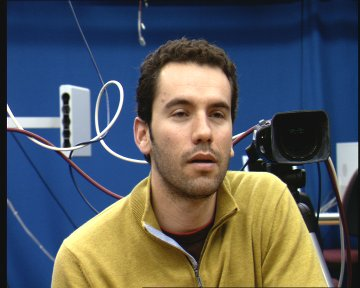
\includegraphics[width = 0.24 \columnwidth]{corpus/3008.jpg}
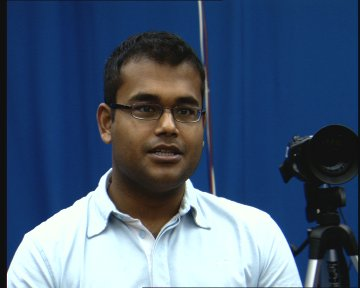
\includegraphics[width = 0.24 \columnwidth]{corpus/3011.jpg}
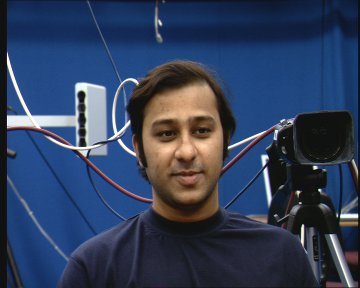
\includegraphics[width = 0.24 \columnwidth]{corpus/6008.jpg}
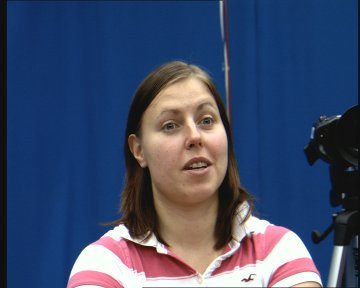
\includegraphics[width = 0.24 \columnwidth]{corpus/6011.jpg}

\caption[An example frame from each of the eight participants.]{An example frame from each of the eight participants. The top row, looking left to right, are participants 1008, 1011, 2008 and 2011. The bottom row are participants 3008, 3011, 6008 and 6011.}
\label{FigureExampleCorpusFrames}
\end{figure}

The laboratory was selected as the setting to perform data capture. This choice was based on the available cameras being directly wired into a fixed, non-portable data recording system. Videos were recorded using two progressive scan, PAL digital video cameras with a frame resolution of 720 by 576 pixels and 25 Hz frame rate. The cameras were arranged to record facial behaviour, which is involved in the expression of many types of \ac{NVC} \cite{Argyle1976} \cite{Morency2011}. The face size in the video was typically around 200 by 300 pixels. The cameras were genlocked to ensure frame synchronisation. The error in synchronisation was smaller than the limits of measurement (a fraction of a microsecond). To minimise synchronisation error, cameras of the same type and synchronisation cables of the same length were used (this ensures the signal propagation from the generator to the cameras takes the same time duration). The arrangement of the lab equipment is shown in Figure \ref{FigureVideoCaptureEquipment}. 
%The resulting video cameras are capable of producing a series of digital frames. 
The corpus was recorded in 2009 and before the availability of affordable consumer depth cameras (which provide both an optical image and a depth map). Recent data sets have begun to utilise ``two and half''{D} or 3{D} recording \cite{Fanelli2010b} with this type of equipment.
%An obvious alternative is to use portable cameras that are battery powered and record to local media.

\begin{figure}
\centering
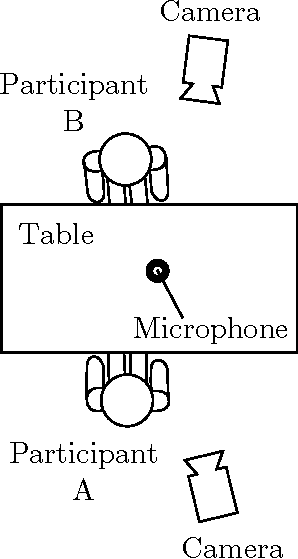
\includegraphics[width = 0.30 \columnwidth]{corpus/VideoCapturePlan.pdf}
\caption{Plan view of video capture equipment arrangement.}
\label{FigureVideoCaptureEquipment}
\end{figure}

Once both participants arrived in the laboratory, they were given only two instructions: to be seated and to communicate until told to stop. Having the participants seated reduces the amount of variation in body and head pose. Without this constraint, participants tend to turn away from the camera which makes facial tracking difficult. The experimenters were not visible to the participants during the recording. The participants were then allowed to talk without further experimenter interaction for 12 minutes. The conversations were of limited duration because the participants may begin to tire and change their behaviour. The instruction to communicate was considered necessary because the laboratory is not a normal place for socialising. The participants seemed to ignore their artificial surroundings and interacted in a natural fashion. The demographics of the participants in the four dyadic conversations are shown in Table \ref{ParticipantDemographics}. The number of conversations and duration was based the need to capture a range of \ac{NVC} behaviours without tiring the participants. The use of eight subjects is suitable for person independent cross validation testing with the majority of the data being available for training (87.5\% in training, 12.5\% in test). Using the person specific \ac{LP} tracker, more individuals and conversations also requires more person specific training to achieve acceptable tracking accuracy and additional resources required to organise and record the corpus. However, more participants results in an increased number of cross validation folds, which allows the standard deviation of the performance to be estimated more accurately. Less individuals in the corpus requires less training data for \ac{LP} tracking (see Appendix \ref{BackgroundLpTracking}), but results in a smaller proportion of data available for training in cross validation. Different cultural pairings were used in each conversation, which rules out the possibility of a study of cultural differences in expression within the TwoTalk corpus. Later chapters consider cultural perception differences, rather than expression differences caused by cultural background. Example frames from the corpus are shown in Figure \ref{FigureExampleCorpusFrames}.

%Samples in the recorded video corpus are informal, unfocused, without pragmatic purpose and topics changes occur in an unstructured way. This fits the description of causal conversation as previous discussed in Section \ref{BackgroundSocialContextUsedInTwoTalk}. 
%Many existing studies use specialised social situations, it is unclear to what extent these findings apply to applications outside the laboratory. Ideally, naturalistic recording of social interactions should take place in their normal location and context. However, it is hoped the near universality and flexibility of informal conversations that they can be recorded in the lab while still having a resemblance to social situations outside the lab.

\diffblock{
\begin{table}
\centering
\caption{Demographics for Conversation Participants in the LILiR TwoTalk Corpus. Abbreviations: UG is an undergraduate degree. M is a master's degree. Certain entries are omitted in cases where the participant was no longer contactable.}
\small
\begin{tabular}{ | c || c | c | c | c | c | c | c |}
\hline
Participant & Country   &  & Age   & Years UK &Education & Languages &  \\
            & of Origin &        & Years & Resident &          & Spoken & Natively \\
\hline
\hline
1008 & Nigeria & \male & 25 & 16 & M  & English & Yes\\
1011 & British & \male & 29 & 25 & UG & English & Yes\\
2008 & Spain   & \male &    &    &                &         & \\
2011 & British & \female  & 27 & 27 & UG & English & Yes\\
     &         &         &    &   &               & French & No \\
     &         &         &    &   &               & British Sign & No \\
3008 & Mexico & \male     & 29 & 5.5 & PhD & Spanish & Yes \\
     &        &           &    &     &     & English & No \\
3011 & Sri Lankan & \male & 25 & 6 & M & Bengali & Yes \\
     &        &          &    &   &             & English   & No \\
     &        &          &    &   &             & Hindi   & No \\
6008 & Indian & \male     & 27 & 1 & M & English & Yes \\
     &        &          &    &   &             & Hindi   & Yes \\
6011 & Ukranian & \female & 27 & 2 & M & Ukrainian & Yes \\
     &          &        &    &   &             & Russian & Yes \\
     &          &        &    &   &             & English & No \\
     &          &        &    &   &             & French & No \\
     &          &        &    &   &             & German & No \normalsize\\
\hline
\end{tabular}
\label{ParticipantDemographics}
\end{table}
}

Four conversations of 12 minutes length provide 48 minutes of conversation. The conversation was recorded by two cameras, resulting in 96 minutes of video. 
%As discussed in Section \ref{BackgroundWhyNvcAnnotationIsBoring}, annotation of \ac{NVC} and emotion is a time consuming and tedious process. 
%Individual \ac{NVC} signals vary from under a second to several seconds or more. 
For multiple annotators, the inter-annotator agreement for corpuses of emotion \cite{Reidsma2008} and \ac{NVC} is low. For this reason, each \ac{NVC} signal clip was rated by multiple annotators to reduce the effect of person specific factors. Much of the recorded conversations contain only passive listening, with no apparent \ac{NVC} displays, which is only marginally interesting. As Cowie \etal \cite{Cowie2009} observed, the distribution of signs is not uniform in human communication. 
%Given these considerations and limitation of resources that could be committed to annotation, the entire video could not be annotated. 
\thesiscomment{QUESTION: To what extent to others manually select a subset of their data? Examples?}
Sections of recordings that contained little or now activity were manually identified and excluded. The remaining sections of video contained potentially interesting behaviours. The annotators were not informed of the particular \ac{NVC} that was potentially present in clips of interest, so the \ac{NVC} content of the corpus was rated entirely by the annotators.
407 clips were selected as potentially of interest. The proportions of \ac{NVC}s that were thought to be present in the initial clip selection process is shown in Figure \ref{FigureManuallySelectedClips}. The different \ac{NVC} frequencies are due to the natural frequencies of occurrence of the various \ac{NVC} signals. An additional 120 randomly selected clips were also included to increase the variety of samples in the corpus. This may include common \ac{NVC} signals that were not considered in the questionnaire and also samples of null \ac{NVC} expression. This increases the richness of the videos shown to the annotators and prevents them reducing the problem to a hard assignment, 4 class problem which may influence the resulting annotation data. Both the manual and random sets of clips are combined, to form a final set of $\numClips=527$ clips with an overall duration of 38 minutes. The clip lengths used ($\lengthofclip=0.6$ to $10$ seconds, average $\overline{\lengthofclip}=4.2s$, standard deviation $\sigma(\lengthofclip)=2.5s$) are similar in duration to Lee and Beattie's work in discourse analysis \cite{Lee1998} (sample lengths of $\overline{\lengthofclip}=4.8s$, standard deviation $\sigma(\lengthofclip)=2.5s$). 
%The clips were presented to the annotators, but without informing them as to what the clip was thought to contain. 
If only total duration is considered, this data set is somewhat smaller than other data corpuses. For example, the emotionally labelled subset of the Belfast Naturalistic Emotional Database has a duration of 86 minutes \cite{DouglasCowie2003}, AMI Meeting corpus has 100 hours \cite{Carletta2007} and Madan's speed dating corpus has 350 minutes \cite{Madan2003}. However, these corpuses have different annotation methodologies and goals, and in many respects are not comparable with the TwoTalk corpus. Canal 9 is a large corpus (42 hours) but only a 10 minute subset is annotated for agreement and disagreement \ac{NVC}.
%Given that there are around 100 positive samples for each category of \ac{NVC} and many more negative samples, we expect that this will be sufficient for training and testing an automatic system.

\thesiscomment{DISCUSS duration of NVC in \cite{Verduyn2009}}

\begin{figure}
\centering
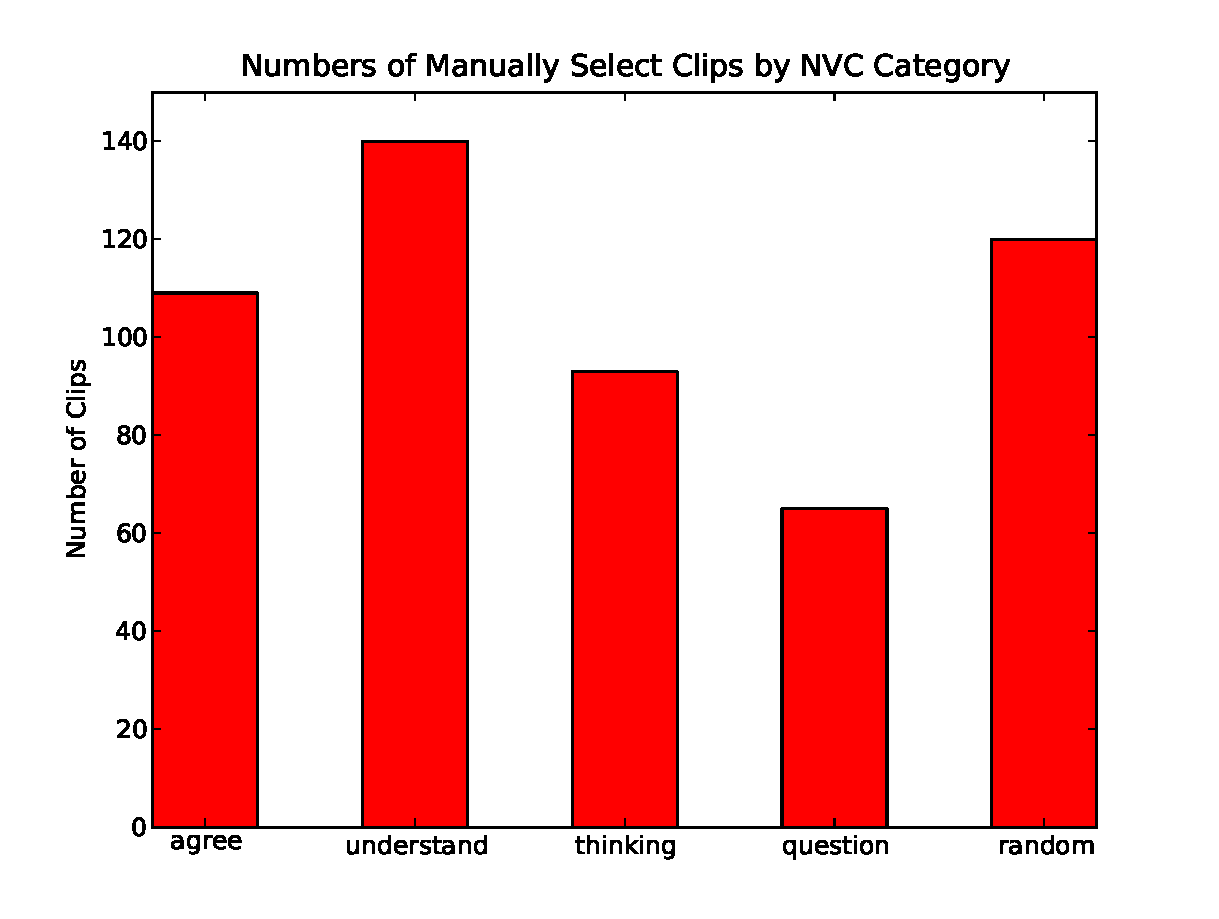
\includegraphics[width = 0.60 \columnwidth]{corpus/FigureManuallySelectedClips.pdf}
\caption[Number of manually selected and randomised clips in each of the NVC categories of interest.]{Number of manually selected and randomised clips in each of the NVC categories of interest. For \textit{agree}, \textit{understand}, \textit{thinking}, \textit{question} and \textit{random}, the number of clips are 109, 140, 93, 65 and 120 respectively.}
\label{FigureManuallySelectedClips}
\end{figure}

\thesiscomment{QUESTION: Several areas for improvement. Location, instructions, social context, selection of participants?}

\thesiscomment{QUESTION: Does changing the balance of clips presented to the user change their perception?}

\section{Design and Description of the Annotation Questionnaire}
\label{SectionSelectionOfNvcCategories}
\label{SectionDescribeQuestions}

%There are many approaches to coding inter-personal corpora.  This section describes the questionnaire used in this study along with a rationale for its design choices.

In attempting to encode \ac{NVC} signals, a system was selected that encompasses as many \ac{NVC} signals as possible, while making the annotation system easy for the annotators to use. In a similar manner to emotion, \ac{NVC} signals change over time and, due to the flexibility of human expression and human interpretation, a vast range of communication signals are possible. 
%An overview of related work is provided in Section \ref{BackgroundQuestionaireDesign}. 
%We use the common assumption that a complex system, \ac{NVC} expression in this case, can be expressed by a combination of more basic components, or in other words, that human communication is a superposition of one or more \ac{NVC} signals. 
However, the specific labels used for \ac{NVC} encoding need to be selected as the basis for annotation. 

%A corpus can be manually encoded based on a description of shape and appearance or in an interpretative sense, which considers the meaning or function of human actions \cite{Kipp2009}. For example, a particular set of muscle contractions (such as \ac{FACS} \cite{Ekman1978} or gaze and Duchenne smiles \cite{Lee1998}) is a descriptive model which can be objectively assessed, in contrast to estimating the intended meaning of a person's gesture which is interpretative. Because many practical applications of \ac{NVC} recognition require an interpretive encoding scheme, this approach is used in this thesis. Of course, it is possible to use descriptive encoding as an intermediate representation, before attempting to recognise interpretative labels and is a complimentary area of study.

An interpretative label is used to encode meaning in \ac{NVC}. An encoding scheme can have a ``categorical'' or ``dimensional'' encoding basis \cite{Cowie2005}. 
%Emotions may also be encoded using appraisal based methods (an observer evaluation determines the true label) \cite{Scherer1999}, but it is unclear if this can be applied to \ac{NVC}. 
Categorical systems rate events based on its similarity to a set of exemplars. Usually these exemplars are based on language that is easy to interpret (e.g. Ekman 6 basic emotions \cite{Ekman1972}). Abstract dimensional systems, which are not based on a simple similarity between an observed to an exemplar expression, attempt to represent a much broader range of events using abstract rating scales. Abstract dimensional encoding includes the commonly used scales activation and valence \cite{Devillers2005}.
%The range of possible meanings conveyed by \ac{NVC} signals is unknown and may be effectively unlimited. This implies that both the categorical and dimensional approach cannot comprehensively encode \ac{NVC}. 
Given the ease of use of exemplar NVC concept labels and the lack of any low dimensional, abstract encoding system for \ac{NVC} encoding, an prototypical (exemplar) \ac{NVC} basis was selected.

%As far as practically possible, categorical encoding of \ac{NVC} should to accurately encode natural conversation. 
Multiple \ac{NVC} signals may occur simultaneously and with a range of intensities. \ac{NVC} encoding needs to address these possibilities. 
%For example, nodding and winking can occur together but can be considered a superposition of nodding and winking. 
For this reason, the popular approach of using multi-class, hard assignment (mutually exclusive) labels is not suitable for capturing the nuances of \ac{NVC} signals. A high dimensional prototypical approach was adopted, which considers \ac{NVC} on multi-dimensional scales \cite{Kruskal1978} which can independently vary. This method is relatively easy to use while accurately encoding a subset of co-occurring \ac{NVC} signals.

%Because the physical actions of \ac{NVC} signals vary in time, the conveyed meaning varies in a similar fashion. 
For temporal annotation of video there are a few approaches that may be used:
\begin{itemize}
 \item One annotation strategy is to evaluate the video using a continuous input device in real time to form a temporally continuous annotation. This thesis considers the issue of temporally continuous to be distinct from being \continuous labels in an \ac{NVC} or emotion dimensional space, however a corpus may possess both properties as in the case of the FeelTrace system \cite{Cowie2000}. Dimensional encoding is typically used for encoding \continuous labels \cite{Nicolaou2011}, although it would be possible in principle to use temporally continuous categorical encoding. Temporally continuous encoding requires  specialised equipment and additional effort by the annotators.
 \item The alternative is to use individual clips rather than long uninterrupted videos. However, this raises the issue of how the start and end frame of clips are selected.
%As discussed in Section \ref{FigureVideoCaptureEquipment}, resource constraints dictated that annotation was performed on a subset of clips. 
\end{itemize}
To control the resources expended in annotation, short clips were manually extracted from the original video recordings and used as the basis for \continuous annotation in this study. This study is therefore not temporally continuous.

%The Ekman basic emotions were not used because this study is concerned with \ac{NVC}, not emotion. 
There is no standardised, comprehensive set of \ac{NVC} signals and little existing research in this area. In one of the few direct studies of \ac{NVC}, Lee and Beattie \cite{Lee1998} examined the use of gaze and Duchenne smiles in an \ac{NVC} context. However these \ac{NVC} signals do not have any obvious practical application. Another study, based on recognizing mental states, was conducted by el Kaliouby and Robinson \cite{ElKaliouby2004}. The mental states they studied were \textit{agreeing}, \textit{concentrating}, \textit{disagreeing}, \textit{interested}, \textit{thinking} and \textit{unsure}. Mental states are not necessarily expressed outwardly and can be expressed with or without communicative intent; this is in contrast to \ac{NVC} which is always communicative, outwardly expressed and intentional. The criteria used in this study for selection of \ac{NVC} signals to study were:

\begin{itemize}
 \item the signal should be an intentional \ac{NVC} action,
 \item they commonly occur in the social context used (i.e. casual chat/informal conversation),
 \item they may be potentially useful in one or more application and
 \item they may modify the meaning of the literal words used.
\end{itemize}

\begin{table}
\centering
\caption{Questions used in web based annotation of the LILiR TwoTalk corpus.}
\begin{tabular}{ | c | c | c | }
\hline
Question for Category & Minimum Rating & Maximum Rating \\
\hline
\hline
Does this person disagree or & Strong  & Strong  \\
agree with what is being said? & disagreement & agreement\\
(A score of 5 is neutral or not applicable.) & & \\
\hline
Is this person thinking hard? & No indication & In deep thought \\
\hline
Is this person asking & No & Definitely \\
a question? & indication & asking question\\
\hline
Is this person indicating they & No indication & Strongly  \\
understand what is being & or N/A & indicating\\
said to them? & & understanding\\
\hline
\end{tabular}
\label{CategoryLabels}
\end{table}

Based on the previous design decisions, the questionnaire is a quantised, multi-dimensional\footnote{Questionnaires can be used to collect multi-dimensional responses e.g. \cite{Tellegen2008}.} encoding using Likert scales of short video clips. The questionnaire presented to the annotators is summarised in Table \ref{CategoryLabels} and reproduced in Appendix \ref{ChapterQuestionnaire}. In this thesis, the 4 categories are abbreviated to \textit{agree}, \textit{thinking}, \textit{question} and \textit{understand}, and refer to the content of this questionnaire. The labels are exemplar based (in a similar fashion to the Ekman basic emotions), unlike activation and valence which are not exemplar based. This thesis uses dimensional labels that are tailored for the needs of \ac{NVC} encoding. As previously discussed in Section \ref{BackgroundQuestionaireDesign}, dimensional encoding is used in a wide variety of human behaviour annotation and is not limited to activation and valence.

As with el Kaliouby and Robinson, the \ac{NVC} labels of \textit{agree} and \textit{disagree} were used because these met the above criteria. Agreement signals are among the most prevalent of \ac{NVC} signals \cite{Bousmalis2009}. Agreement and disagreement are mutually exclusive messages, therefore these labels are expressed on a single dimensional scale. 
%This was later realised to be unnecessary because disagreement was rarely seen in the corpus and are discarded for the purposes of classification. However, other social situations may have frequent expressions of disagreement. 
The \ac{NVC} signal \textit{thinking} was used because it is a common and distinct behaviour in the corpus, based on an informal viewing of the corpus videos. Also, the tracking method used is very effective for eye movements and gaze is known to play a role in conversation turn taking \cite{Argyle1976}. The way gaze varies during thinking is culturally dependent \cite{McCarthy2006}, making it a potentially interesting \ac{NVC} signal when comparing different cultural perceptions of \ac{NVC} (see Chapter \ref{ChapterNvcRegression}). However, \textit{thinking} is arguably a mental state, as much as a true communication signal. 
%However, it is associated with a facial gesture which may be an intentional action to regulate the conversation.
 \textit{Question} is included because it drastically changes the meaning of an utterance, which may have applications in multi-modal speech recognition. The inclusion of \textit{question} was debatable, because while questions can be recognised by changes in voice intonation, it was unknown if visual recognition of a question was even possible. \textit{Understand} is another common signal which regulates conversation and has both verbal and non-verbal components. 
%The number of \ac{NVC} signals studied was limited because of the limited resources available for annotation of the data. 
The \ac{NVC} signals of \textit{agree} and \textit{understand} express attitudes and are therefore social signals. While \textit{thinking} and \textit{question} are likely to have a role in regulating conversation flow, their exact role and significance is uncertain and their status as social signals is current uncertain.

A questionnaire can collect dimensional responses may have labels values that are either discrete (quantised) or continuous. Continuous value data may be collected by marking a point on a continuous line using either a written mark or computer input \cite{Treiblmaier2011}. The term ``continuous value'' does not exclusively apply to annotations with continuous temporal traces, such as FeelTrace\footnote{Human behaviour may either be encoded as either discretised or continuous in terms of annotation labels: ``When discretised dimensional annotation is adopted (as opposed to continuous one), researchers seem to use different intensity levels'' \cite{Gunes2011}}. The concept of ``continuous emotional space'' is expanding beyond activation and valence, with Hupont \etal \cite{Hupont2013} using a 2{D} continuous value space (\textit{evaluation} and \textit{activation}) without considering the temporal dimension. Liscombe \etal \cite{Liscombe2003} used a web-based survey to gather \continuous emotion annotation data for each utterance in an audio corpus. Discrete binary labels might simply be ``\ac{NVC} is expressed'' and ``\ac{NVC} is not expressed''. Binary discrete labels were used by Lee and Beattie \cite{Lee1998} in their discourse analysis of \ac{NVC}. Discrete labels can also be used in dimensional annotation and may be encoded using integer values. Continuous valued labels are dimensional ratings that have non-integer values and are commonly used in psychological research \cite{Nicolaou2011, Wollmer2009, Cowie2000}. A Likert scale \cite{Likert1932} is a common psychometric questionnaire in which a ordinal rating can be provided between two extreme choices. Taking the mean of multiple annotators results in a value that can take non-integer values and is therefore a \continuous variable. While some concerns have been raise as to the validity of using a Likert scale as an interval-level measure with parametric statistics \cite{Jamieson2004}, a number of studies have examined the use of Likert scales as an interval-level measure and found it to be a reliable research tool \cite{Rasmussen1989} \cite{Owuor2001}. Both Carifio and Perla \cite{Carifio2007} and Norman \cite{Norman2010} argue that it is time to put the controversy of the use of the Likert scale as a interval-level measure in the past because of the repeated demonstration of the worth of using Likert scales with parametric statistics, such as mean and variance.
%A binary label is less expressive than a continuous scale. 
%A continuous scale was used to avoid losing information that may be relevant to a practical application. However, 
A Likert scale was used in this study as this retains intermediate intensity expressions while being applicable to an Internet based survey.

%This section has described the TwoTalk corpus and questionnaire. The following section describes how the annotation data was collected.

\section{Multi-observer Annotation of NVC}
\label{SectionMultiCultitureAnnotation}

%The previous sections have described how the questionnaire was designed and how the data corpus was recorded. 
%To use supervised learning on this corpus, the sample labels need to be determined.
Inter-annotator agreement for inter-personal events is typically low. (``These annotations [of subjective corpura] often have a quite low overall level of inter-annotator agreement'' \cite{Reidsma2008}) This is also likely to be true for \ac{NVC} perception. \ac{NVC} perception is highly subjective and partly dependent on person specific, social and cultural factors (see Section \ref{BackgroundWhatFactorsInfluenceNvc}). Multiple annotators are used in an attempt to reduce the effect of interpersonal variations. Other techniques to improve inter-annotator agreement were not employed (e.g training the annotators, having the annotator previewing the corpus, multiple ratings on individual clips by individual annotators, subject normalisation). This was due to the limitations in resources needed to conduct such a study and the technical limitations of crowd sourced annotation.
The differences in perception between cultures are not considered in this chapter, but this issue is revisited in Chapter \ref{ChapterAnnotation}.

\begin{figure}[tb]
\centering
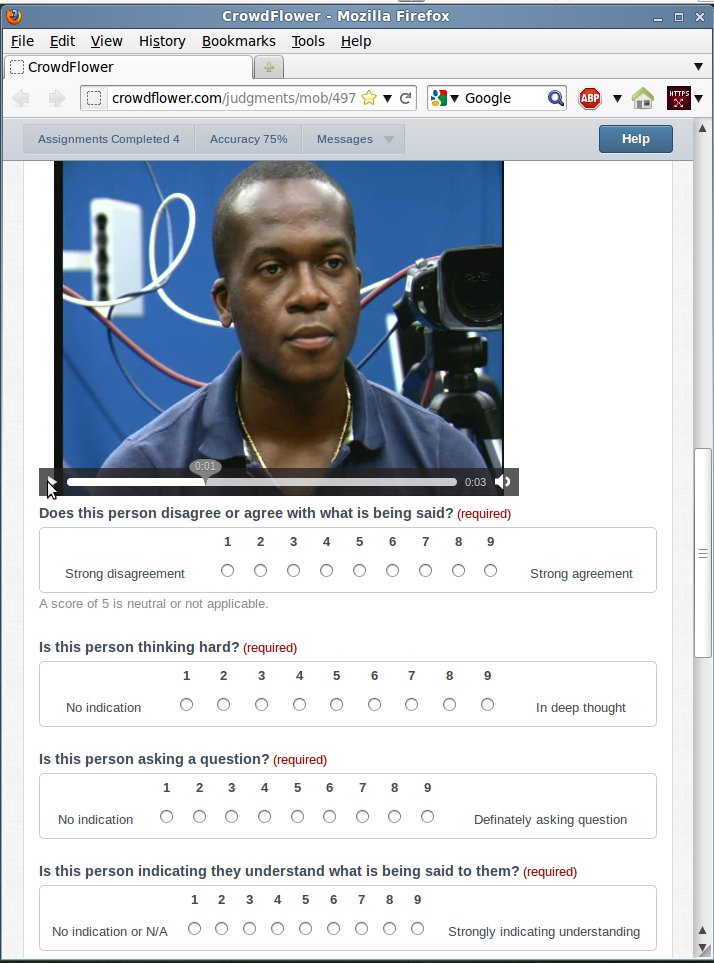
\includegraphics[width = 0.5 \columnwidth]{corpus/crowdflower-survey.png}
\caption[A typical page of the annotation questionnaire, which is accessed using a web browser.]{A typical page of the annotation questionnaire, which is accessed using a web browser. Each clip is annotated individually. The user has the ability to replay the video and is required to respond to the four \ac{NVC} questions.}
\label{FigureAnnotationSurveyScreenshot}
\end{figure}

The questionnaire was presented to annotators using a computer based system. These are commonly used for annotation of video \cite{Eckhardt2009, Cowie2000, Tarasov2010} and allow participants to complete the survey at their own convenience, rather than having to attend an organised session. A web based system was used, because the system could be remotely accessed using a web browser. A web page displayed one or more videos and each could be viewed one or more times. Under each video were the four annotation \ac{NVC} categories selected in Section \ref{SectionDescribeQuestions}. The user viewed the video clip and marked their answer using the mouse or keyboard. The order of the videos was randomised to reduce the possible effect of the video display order on the annotation data. A typical view of the annotation web site is shown in Figure \ref{FigureAnnotationSurveyScreenshot}. The videos were presented to the annotators with both visual and audio information. By presenting both, it was hoped that the most natural and realistic rating would be achieved. 
%Most, but not all \ac{NVC} information expressed in the visual domain (see Section \ref{BackgroundHowIsNvcExpressed}). 
%For this reason the automatic systems discussed in this thesis use visual information only. 
%Since not all the information that might be relevant to determining what \ac{NVC} is present, it might be expected that the automatic system will have some difficulty in correctly identifying types of \ac{NVC} that rely on an audio component (e.g. \textit{question}).

Allowing users to perform the annotation task with no supervision risks the participants not completing the annotation task as instructed.
%, for example having the audio disabled when rating the videos. 
The annotators were unpaid volunteers and were motivated by interest, loyalty or duty and were expected to generate relatively good quality data. Another approach used is to pay people to perform the annotation but this can lead to quality issues, which are addressed in Section \ref{SectionNeedToFilter}. Chapter \ref{ChapterAnnotation} addresses collecting annotation data from observes based in different cultures.

%Once the annotation system was designed and implemented, annotators began to view and rate examples of \ac{NVC} signals. The next section provides an analysis of their responses.

\section{Analysis of Human Annotators}
\label{SectionAnalysisOfHumanAnnotation}

\begin{figure}[tb]
\centering
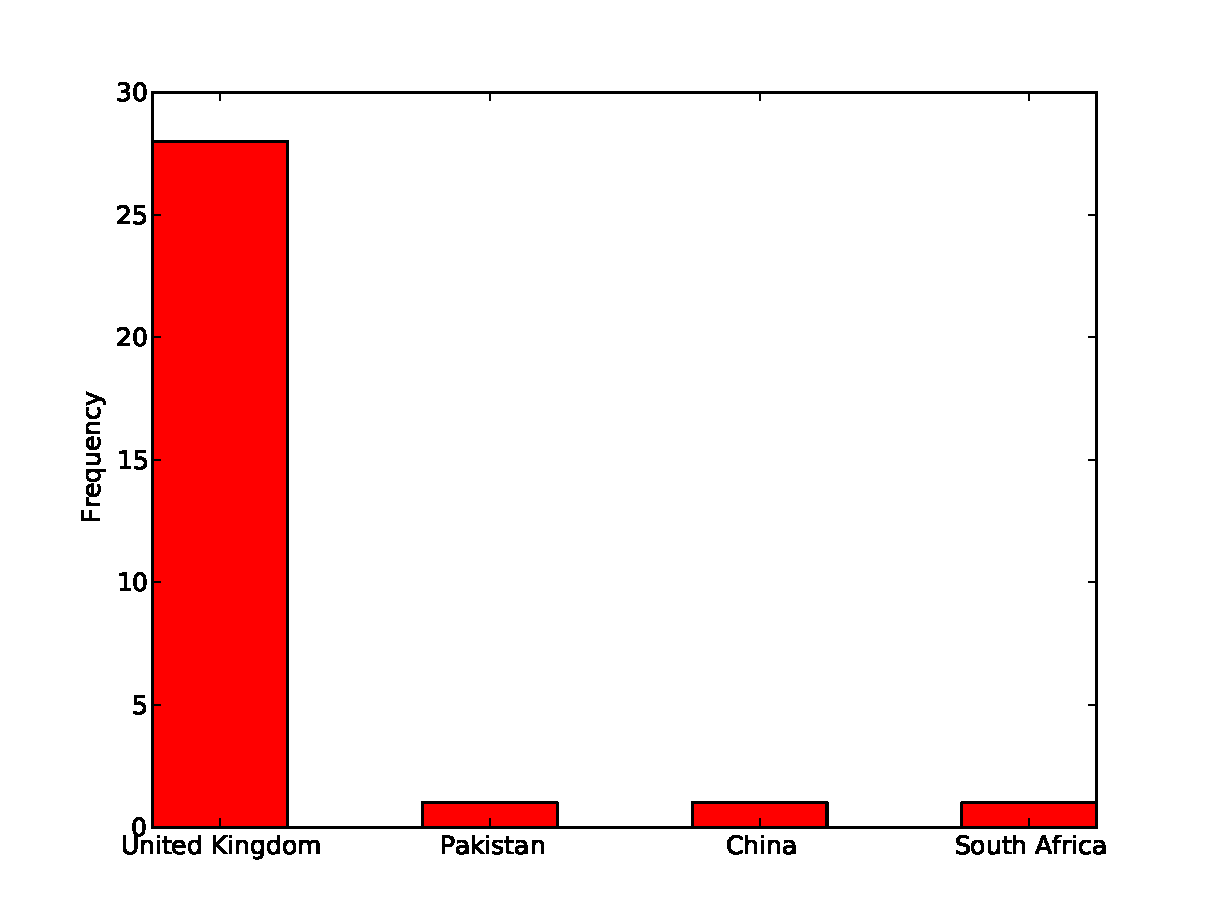
\includegraphics[width = 0.5 \columnwidth]{corpus/demographicLocation.pdf}
\caption{Self-reported primary culture for annotators.}
\label{FigureDemographicLocation}
\end{figure}

Thirty one annotators participated in rating samples of \ac{NVC} ($\numAnnotators = 31$). Because expression and perception is dependent on cultural context, gender and personality differences (see Section \ref{BackgroundWhatFactorsInfluenceNvc}), it is relevant to consider the demographics of the annotators. Although all annotators were UK residents, some annotators had a separate primary cultural background. Annotators were mostly 21-30 years of age, with a science or engineering background (see Figure \ref{FigureDemographicAge} and \ref{FigureDemographicWork}). As can be seen in Figure \ref{FigureDemographicLocation}, the vast majority of annotators had a UK based cultural background. 
%Considering this, and the other annotators exposure to UK culture, it is likely that the cultural background of the annotators will only be a minor factor in any differences between annotators. However, the annotation data collected is from a single cultural perspective.
Annotation by distinct cultural groups is discussed in Chapter \ref{ChapterAnnotation}. The majority of respondents were male (see Figure \ref{FigureDemographicGender}). 
%The existence of two distinct groups among the annotators, each having a different perception of \ac{NVC} signals, might lead to two distinct clusters of annotation results. 
%The next section discusses how this may be reduced to a simple label. 
%The demographic questionnaire also asked about the annotators field of work. 
%Terracciano \etal \cite{Terracciano2003} found there is a relationship between personality and emotion perception. The role of personality is thought to influence the choice of career, although that role not well understood \cite{Vuust2010}. 
%It would be interesting to discover if there is a connection between \ac{NVC} perception based on career. 
It might be beneficial to include a personality questionnaire in future annotation projects to enable investigation of personality in a more explicit way. %The \ac{NVC} ratings provided by the annotators will now be considered.

\begin{figure}[tb]
\centering
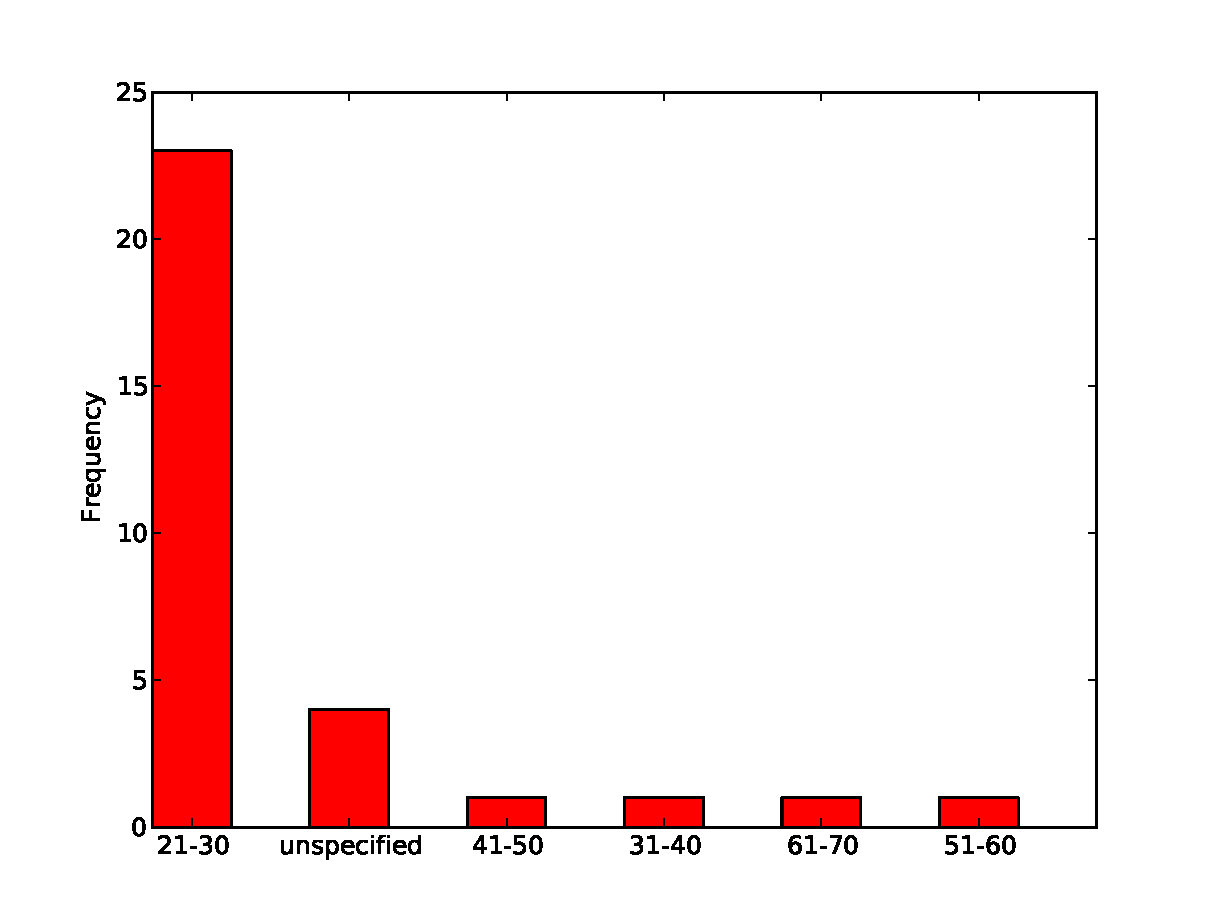
\includegraphics[width = 0.60 \columnwidth]{corpus/demographicAge.pdf}
\caption{Self-reported age for annotators.}
\label{FigureDemographicAge}
\end{figure}

\begin{figure}[tb]
\centering
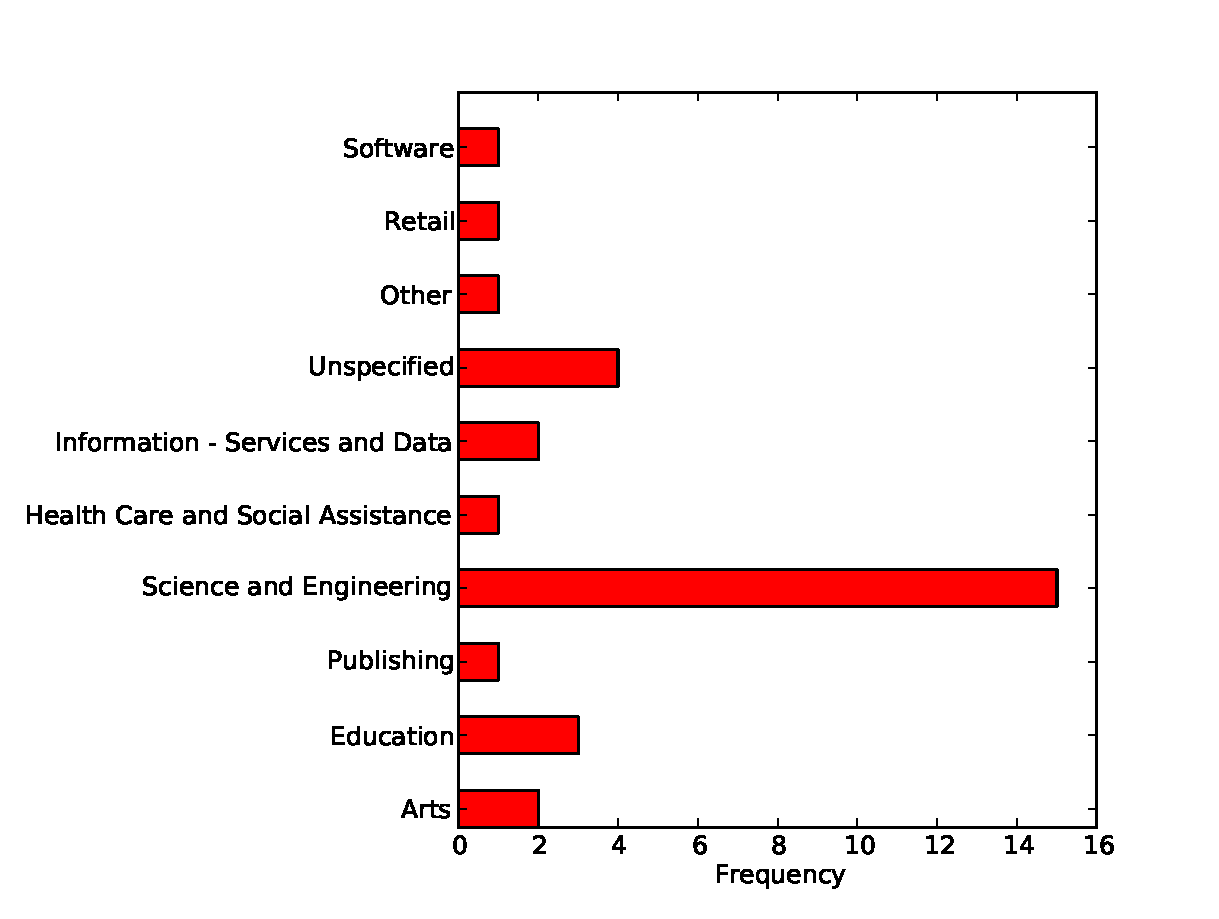
\includegraphics[width = 0.60 \columnwidth]{corpus/demographicWork.pdf}
\caption{Self-reported sector of employment for annotators.}
\label{FigureDemographicWork}
\end{figure}

\begin{figure}[tb]
\centering
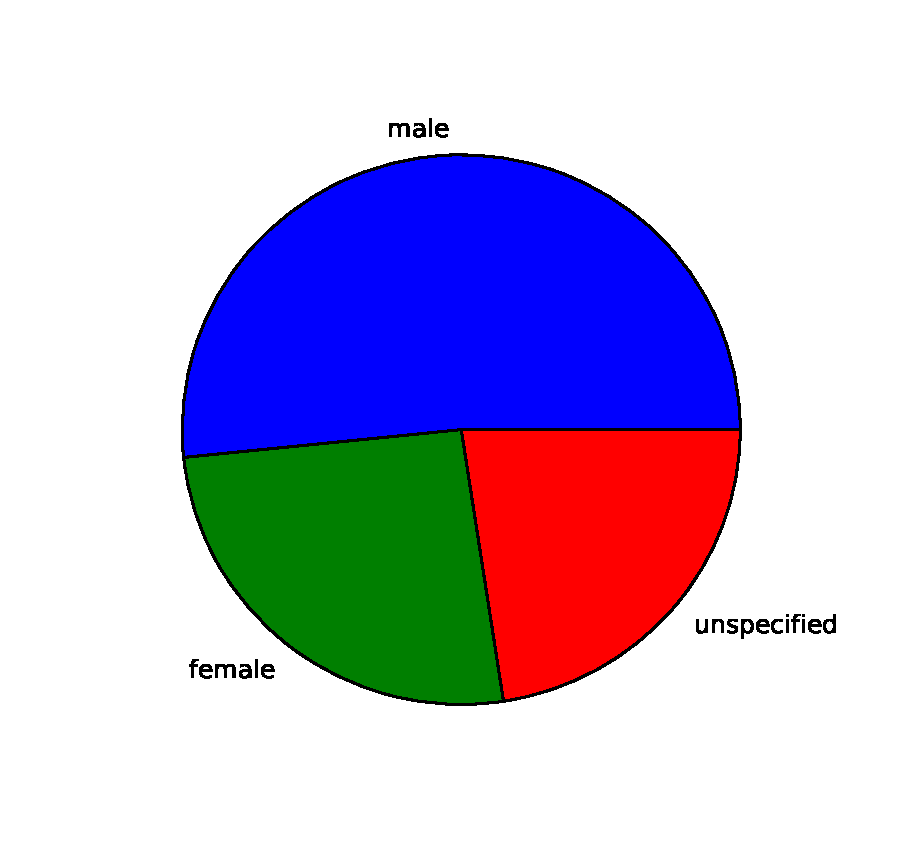
\includegraphics[width = 0.5 \columnwidth]{corpus/demographicGender.pdf}
\caption{Self-reported gender for annotators.}
\label{FigureDemographicGender}
\end{figure}

The vast majority of annotators did not rate every video clip because \ac{NVC} annotation is time consuming and tedious. On average, each annotator rated 70 video clips, from a possible maximum of 527 clips. Each clip required all four \ac{NVC} signals to be rated. For the \ac{NVC} category \textit{thinking}, 2182 individual ratings were provided by the annotators, distributed across the corpus's 527 video clips. This corresponds to 4.1 ratings per video clip. 
%Having multiple ratings on a single question on a single \ac{NVC} video clip should reduce the effect of person specific \ac{NVC} perception. The other \ac{NVC} signals had a similar level of response. 

\begin{figure}[tb]
\centering
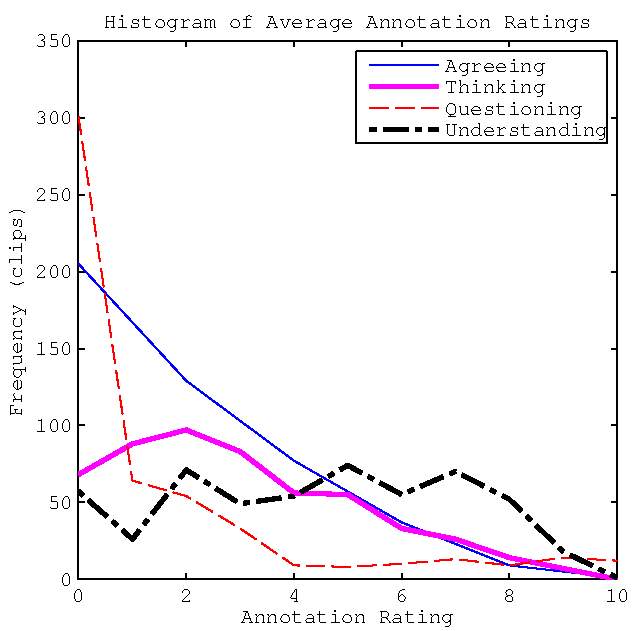
\includegraphics[width = 0.5 \columnwidth]{corpus/ratingof4.pdf}
\caption[Histogram of Average Rating based on multi-annotators.]{Histogram of Average Rating based on multi-annotators. Blue thin line is agreeing, magenta thick line is thinking, black dot-dashed line is understanding and red dashed line is questioning. Zero is a neutral score and 10 is strongly showing the communication signal. Disagreement ratings have been omitted.}
\label{RatingScoresFigure}
\end{figure}

%The questionnaire considers \ac{NVC} signals as varying in intensity from strongly showing a signal to no indication of an \ac{NVC} signal. The ratings were provided on a pseudo-continuous scale with intermediate intensity emotions receiving a score between extremes. 
Not all \ac{NVC} signs occur with the same frequency or intensity. Figure \ref{RatingScoresFigure} shows the distribution of \ac{NVC} intensity for the annotated videos. The frequency of \ac{NVC} occurrence in these videos almost certainly differs from unedited video, because the video clips in the corpus were specifically selected to include interesting \ac{NVC} examples and to avoid inactive sections. \textit{Question} \ac{NVC} has a strong peak at zero, indicating the majority of video clips do not contain this signal. 
%This is unsurprising, because the manually selected clips had relatively few examples of \textit{question} \ac{NVC} (see Figure \ref{FigureManuallySelectedClips}). 
\textit{Agree} and \textit{thinking} \ac{NVC} have a similar peak near ``no \ac{NVC} signal'', but differ from \textit{question} by having a minority of clips of intermediate intensity. \textit{Understand} \ac{NVC} has a relatively uniform frequency distribution, with some weak, intermediate and strong examples. Intense expression is rare for the \ac{NVC} signals considered in this work. Combining multiple individual annotator ratings to a single vector label will now be considered.

\section{Analysis of Mean Ratings}
\label{SectionAnalysisOfMeanRatings}

Annotator ratings are provided for each of the \ac{NVC} categories:

\begin{align}
\nvcCategory \in \setCategories = \{agree, understand, think, question\}
\end{align}

%For each video clip, the annotation produces a set of ratings for each \ac{NVC} category. 
%The number of annotator ratings is variable, however the supervised learning paradigm assumes each sample has a single label. 
For supervised learning, the individual ratings need to be reduced to a single consensus 4{D} label for each clip. This is performed by taking each \ac{NVC} quantised, dimensional rating and calculating the mean (similar to \cite{Tarasov2010, Wollmer2009}), which results in a \continuous label. The vector containing the number of annotation ratings for $\numClips$ clips is defined as $\numAnnotatorsOnClip \in \mathbb{N}^{\numClips}$. The ratings for clip $\clipId \in \{1...\numClips\}$, annotated for \ac{NVC} signal category $\nvcCategory$, is designated as matrix $\rawAnnotation_{\nvcCategory,\clipId}$ of size ${4 \times \numClips}$. $\rawAnnotation_{\nvcCategory,\clipId}$ comprises of a set of tuples, containing ratings $\ratingOfClip_i \in \mathbb{R}$ and corresponding annotator indices $\annotatorOfRating_i \in \{1...\numAnnotators\}$:
%($i \in \numAnnotatorsOnClip_{\clipId}$)
%$\rawAnnotation^{\nvcCategory}_{\clipId} \in \mathbb{R}^{\numAnnotatorsOnClip_{\clipId}}$
\begin{align}
\rawAnnotation_{\nvcCategory,\clipId} = \{(\ratingOfClip_i, \annotatorOfRating_i)\}_{i=1}^{\numAnnotatorsOnClip_{\clipId}}
\end{align}

The 4 \ac{NVC} categories and can be summarised into a consensus vector $\clipConcensus \in \mathbb{R}^{4 \times \numClips}$, $\nvcCategory \in \setCategories$:

\begin{align}
\clipConcensus_{\nvcCategory, \clipId} = \frac{\displaystyle\sum\limits_{i=1}^{\numAnnotatorsOnClip_{\clipId}} \{\ratingOfClip_i: (\ratingOfClip_i, \annotatorOfRating_i) \in \rawAnnotation_{\nvcCategory,\clipId}\}}{\numAnnotatorsOnClip_{\clipId}}
\end{align}

%For a specific clip, a four \ac{NVC} category consensus rating is found:

%\begin{align}
%\clipConcensus(\rawAnnotation)_{\clipId} = [\clipConcensus(\rawAnnotation)^{agree}_{\clipId}, \clipConcensus(\rawAnnotation)^{understand}_{\clipId}, \clipConcensus(\rawAnnotation)^{thinking}_{\clipId}, \clipConcensus(\rawAnnotation)^{question}_{\clipId}]
%\end{align}

This simplification assumes that inter-annotator differences are not significant for the intended application and that the annotator ratings are symmetrically distributed. However, human perception of \ac{NVC} depends on many factors (see Section \ref{BackgroundWhatFactorsInfluenceNvc}). The bulk of this thesis attempts to create and evaluate an automatic system that produces a prediction in a similar fashion to a human annotator. This chapter assumes the annotators form an approximately self-consistent group because of the demographic similarity of the annotators (see Section \ref{SectionAnalysisOfHumanAnnotation}).
% and any deviations in annotation are approximately symmetrically distributed. 
Therefore, using the rating mean to determine a consensus is valid in this case. However, it is important to remember the limitations of using the mean consensus, and specifically that taking the mean of non-homogeneous groups risks over-simplification of the problem. Chapter \ref{ChapterNvcRegression} considers the case of training an automatic system when multiple distinct groups of annotators exist.

An alternative to using the mean rating is to take a set of multiple annotator rating data and use a subset of clips in which there is agreement, as done by el Kaliouby and Robinson \cite{ElKaliouby2004}. This approach was not used, because it ignores clips in which there is low inter-annotator agreement.
%, but a broad coverage - including hard to rate clips - may be important for any practical application. The issue of dealing with separate annotator groups is raised in Chapter \ref{ChapterAnnotation}, as well as examine the case for treating cultures as separate label sets.

\begin{table}[tb]
\centering
\begin{tabular}{ | c || c | c | c | c | }
\hline
& Agreeing & Understanding & Thinking & Questioning \\
\hline
\hline
Agree & 1 & & &\\
Understand & 0.46 & 1 & &\\
Thinking & -0.21 & -0.23 & 1 &\\
Question & -0.18 & -0.40 & 0.06 & 1 \\
\hline  
\end{tabular}
\caption{Correlation coefficients of the mean ratings $\clipConcensus$ for each category.}
\label{CorrelationOfCategoriesTable}
\end{table}

%As discussed in Section \ref{SectionSelectionOfNvcCategories}, we treat the expression of complex \ac{NVC} as a superposition of more basic \ac{NVC} signals. However, 
The selected \ac{NVC} categories do not necessarily vary independently of each other. A linear dependence of two continuously varying signals can be found by calculating the Pearson correlation coefficient $\correlFunc$. The Pearson correlation coefficient $\rho$ for vectors $\textbf{x} \in \mathbb{R}^{n}$ and $\textbf{y} \in \mathbb{R}^{n}$, is defined as (adapted from \cite{Weisstein2008}, for a population, $i=\{1..n\}$):

\begin{gather}
\correlTemp(\textbf{x},\textbf{x}) = \displaystyle\sum\limits_{i=0}^n {\textbf{x}_i}^2 - n\bar{\textbf{x}}^2\\
\correlTemp(\textbf{y},\textbf{y}) = \displaystyle\sum\limits_{i=0}^n {\textbf{y}_i}^2 - n\bar{\textbf{y}}^2\\
\correlTemp(\textbf{x},\textbf{y}) = \displaystyle\sum\limits_{i=0}^n {\textbf{x}_i \textbf{y}_i} - n\bar{\textbf{x}}\bar{\textbf{y}}\\
\correlFunc (\textbf{x},\textbf{y})^2 = \frac{{\correlTemp(\textbf{x},\textbf{y})}^2}{\correlTemp(\textbf{x},\textbf{x}) \correlTemp(\textbf{y},\textbf{y})}
\label{EqnPearsonsCorrelation}
\end{gather}

\thesisstatement{Some pairs NVC category annotator responses are correlated}

where $\bar{\textbf{x}}$ and $\bar{\textbf{y}}$ are the mean values of $\textbf{x}$ and $\textbf{y}$ respectively. The value of $\rho$ gives an indication of the correlation between two signals. $\rho=1$ is perfect positive correlation, $\rho=0$ indicates no correlation and $\rho=-1$ indicates perfect negative correlation. The correlation between different \ac{NVC} signals is shown in Table \ref{CorrelationOfCategoriesTable}. The highest magnitude correlation score is between \textit{agree} and \textit{understand}, with a score of $\rho=0.46$. This is a relatively weak correlation but significant enough to say there is a relationship between these signs. This also confirms our intuitive expectation, because if a person wishes to indicate agreement, this necessarily implies they also want to convey that they understand. The next highest magnitude score is for \textit{understand} and \textit{question} at $\rho=-.40$. Being a negative correlation, this reflects that these signals are partially mutually exclusive; when a person is asking a question, they are unlikely to be conveying that they understand (and visa versa). Finally, the lowest magnitude score is for \textit{thinking} and \textit{question}, having a correlation of $\rho=0.06$. This implies these \ac{NVC} signals occur relatively independently of each other.

This analysis is interesting, because if there are many \ac{NVC} signals that are interrelated, it can imply that dimensionality reducing techniques can be applied without loss of information. 
%However, only a limited subset of \ac{NVC} signals is considered, so dimensional reduction of labels is not attempted in this work. Also, knowing which \ac{NVC} signals are independent and which are mutually exclusive is different from a multiclass approach, which assumes every class is mutually exclusive. 
The \ac{NVC} signals \textit{agree} and \textit{understand} often co-occur, therefore an approach using a single discrete class label would be problematic for \ac{NVC} recognition.

\thesiscomment{DISCUSS Equate neutral expression with no NVC being sent? Show examples? What about the possibility of sending NVCs not included in this study during inactivity?}

%This section has discussed the annotations and demographics provided by the volunteers. The next section concludes this chapter and outlines how it will be used for supervised learning.

\thesiscomment{QUESTION: Run our online tracker on these sequences? It should fail?}

\begin{figure}[tb]
\centering
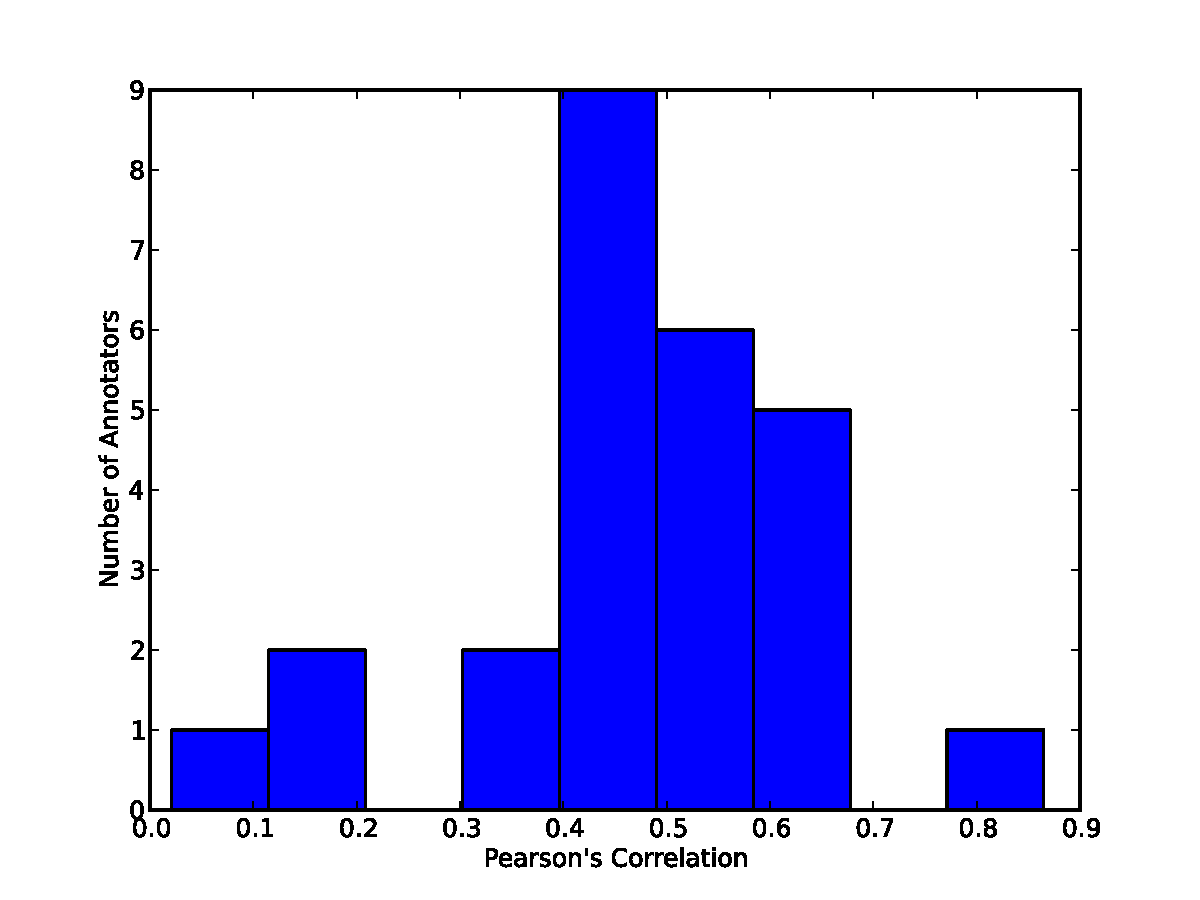
\includegraphics[width = 0.80 \columnwidth]{corpus/AnnotatorCorrelHist.pdf}
\caption{A histogram of Pearson's correlation between an annotator's ratings and the mean of all other annotators' ratings. Some annotators did not rate enough data to compute a valid correlation and were excluded from this figure.}
\label{FigureAnnotatorCorrelationWithConc}
\end{figure}

The ratings for each annotator are compared to the mean of the other annotators. This provides a measurement of inter-annotator agreement. Figure \ref{FigureAnnotatorCorrelationWithConc} shows a histogram of the number of annotators at different levels of agreement with the cultural consensus. This shows that some annotators are in close agreement with the cultural consensus, while others are less so. For all 31 annotators, the average correlation with consensus is $0.47$. Inter-annotator agreement is discussed again in Section \ref{SectionAnnotationFilterMethod} in context of removing outlier annotators.

Correlation is used as the primary measurement of agreement of survey data in this study. The use of the popular Cronbach's Alpha is not a suitable measure of agreement or internal consistency \cite{Sijtsma2009, Revelle2009, Sijtsma2009b}, with Green and Yang calling for it's general use should be discouraged \cite{Green2009}. This metric is therefore not used in this thesis. Also, the habitual use of a particular threshold (such as the commonly used value of 0.7 or 0.8) to determine if a questionnaire validity risks over-emphasising the problem of random noise, to which machine learning techniques are somewhat robust, and ignoring the problem of systematic errors by the annotators (See Chapter 3 of Reidsma \cite{Reidsma2008Thesis}). Reidsma argued that using corpus data with a higher inter-annotator agreement generally leads to better performance in automatic recognition.

\section{Conclusion}

This section has described a corpus that comprises of recordings of two person, informal conversations. Minimal experimental constraints were used to maximised the natural and spontaneous character of the social situation. Annotation was performed on video clips to encode the conversation meaning. The annotators were shown the video clips with audio. The data was collected based on quantised, dimensional Likert questions. Based on this, a consensus label based of the mean of multiple annotators was calculated for each question which resulted in \continuous labels. This consensus annotation data will be used in later chapters of this thesis as the basis for an automatic system.

Currently, the cultural background of the \ac{NVC} encoders and the annotators is not well controlled. To understand and distinguish between personal and cultural differences, it would be beneficial to have recordings from distinct cultures and have them annotated by multiple cultures. 
%The corpus can then be analysed to find the different usages and frequencies of \ac{NVC} gesture. Also, cultural differences in perception of \ac{NVC} signals can be examined. 
This use of culturally distinct annotators is discussed in Chapter \ref{ChapterAnnotation}.

The finding that \ac{NVC} labels often co-occur and do not vary independently raises the question as to redundant information in \ac{NVC} labels. If \ac{NVC} can be expressed in a lower dimensional space, the annotation task and automatic recognition problem are both simplified. However, the \ac{NVC} labels used are not comprehensive and further work is needed to find an \ac{NVC} annotation system with a broader coverage of meaning.

The corpus was recorded in a laboratory environment. It is likely that more naturalistic data would be obtained by recording data in an environment in which an automatic system is expected to be deployed. Some data sets that attempt this have recently become available, such as the D64 Multimodal Conversational Corpus being recorded in a domestic environment. %When an automatic system is trained on data that is representative of an application, it will have improved performance.
The next chapter describes an automatic \ac{NVC} classification system based on the data collected in this chapter.
